\section {Arena Specification}

\subsection {Arena Dimensions}
\label{arena}

\begin {description}
\item [\ref{arena}.1] Robots will compete in a arena of 12 x 8m and 0.6m height.
\item [\ref{arena}.2] Entrance and exit to arena will only be made via the entrance and exit doors respectively.
\item [\ref{arena}.3] No person is permitted in the arena whilst robots are active.
\item [\ref{arena}.4] No person is allowed in the arena until permitted by an event official.
\end {description}

\subsection {General Layout}
\label{arenagenlay}

\begin {figure}[h]
\begin {center}
\includegraphics[keepaspectratio, scale =0.65]{../arena/arena.png}
\caption{\small{\emph{The General Arena Layout}}}
\label {fig:arena}
\end {center}
\end {figure}

\subsection {Tokens}
\label{tokens}

\begin {description} 
%\item [\ref{tokens}.1] Robots must collect tokens in order to achieve points.
\item [\ref{tokens}.1] Tokens will be cylindrical of 100mm length and 40mm diameter.
\item [\ref{tokens}.2] A token only accounts to a team's score when it is successfully placed in a zone. The token must be touching the zone floor in order to count.
\item [\ref{tokens}.3] Robots should not intentionally damage or destroy tokens.
\end {description}

